\documentclass[aspectratio=169]{beamer}

\usepackage[english]{babel}
\usepackage{graphicx}
\usepackage{media9}
\usepackage[absolute, overlay]{textpos}
\usepackage{multicol}
\usepackage{tikz}

\usetikzlibrary{arrows, decorations.markings}

\usetheme{Madrid}
\usecolortheme{crane}
\setbeamertemplate{page number in head/foot}{}
\setbeamertemplate{navigation symbols}{}

\title[Automatic Generation of Safety-Critical Test Scenarios]{Automatic Generation of Safety-Critical Test Scenarios\\for Collision Avoidance of Road Vehicles\\by Matthias Althoff and Sebastian Lutz}
\author{Stefan Huber}
\institute{University of Passau}
\date{\today}
\titlegraphic{
\includegraphics[height=.10\textheight]{media/logoUniPassau.jpg}}

\newcommand{\includeFSVideo}[1]{%
    \begin{textblock*}{5pt} (0pt, 0pt)
        \includemedia[
            height=\paperheight,
            width=\paperwidth,
            addresource=#1,
            activate=pageopen,
            playbutton=none,
            flashvars={source=#1&autoPlay=true&loop=true}
        ]{}{VPlayer9.swf}
    \end{textblock*}
}

\newcommand{\videoframe}[1]{%
    \begin{frame}[plain]
        \includeFSVideo{#1}
    \end{frame}
}

\newcommand{\fsFrame}[1]{%
    \begin{frame}[plain]
        \centering
        \Huge{#1}
    \end{frame}
}

\begin{document}

\begin{frame}[plain]
    \noindent\makebox[\textwidth]{%
        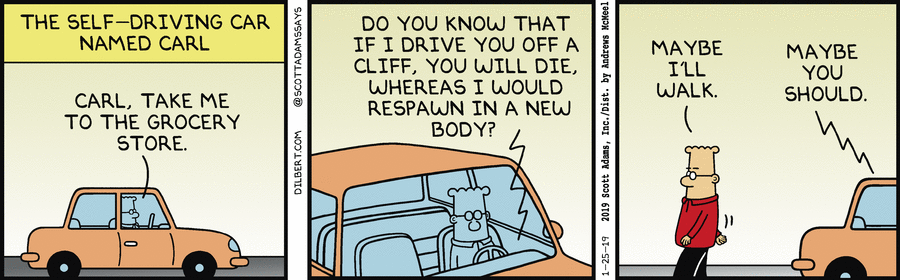
\includegraphics[width=.97\paperwidth]{media/2019-01-25_dilbert_autonomousCars.png}
    }
\end{frame}

\maketitle

\videoframe{media/2019-02-21_BasicUnoptimizedScenario.mp4} % Motivate

\begin{frame}{Differentiation to other approaches}
    \pause%
    \begin{tikzpicture}
        \node[anchor=south west, inner sep=0] at (0,1) {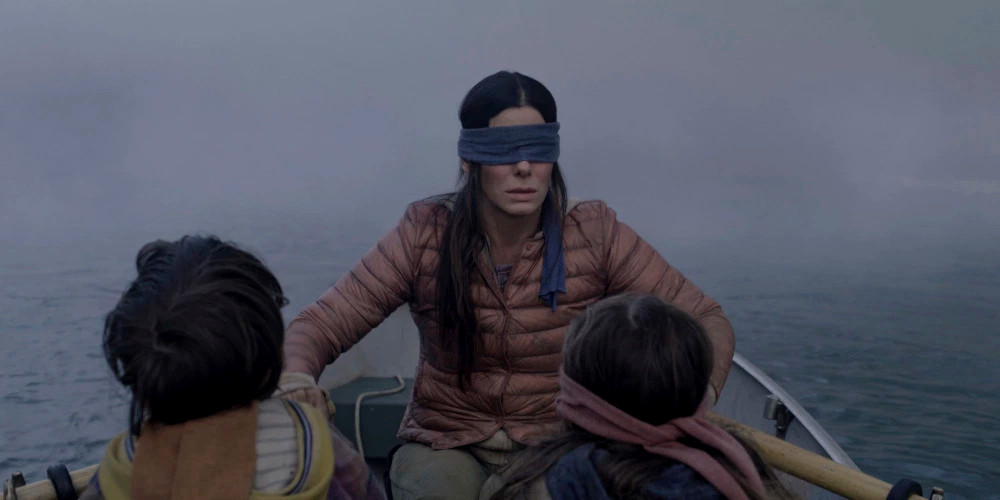
\includegraphics[width=.6\textwidth, trim=80 0 180 0, clip]{media/birdBox.jpg}};
        \node[draw=none] at (3,7.5) {Other approaches};

        \onslide<3->{%
            \node[anchor=south west, inner sep=0] at (7,1.2) {
\includegraphics[width=.6\textwidth]{media/construction.png}};
            \node[draw=none] at (11.2,7.5) {This approach};
            \draw[red, line width=0.8mm, line cap=round] (0,1.5) -- (6.5,7) {};
            \draw[red, line width=0.8mm, line cap=round] (0,7) -- (6.5,1.5) {};
            \draw [->, red, line width=7mm, >=stealth] (5.5,4) -- (9,4) {};
        }
    \end{tikzpicture}
\end{frame}

\videoframe{media/drivableArea_slow.mp4}
\videoframe{media/drivableArea_fast.mp4}

\fsFrame{Limit 50 km/h}
\videoframe{media/beamNG_toSlow.mp4}
\fsFrame{Limit 70 km/h}
\videoframe{media/beamNG_adequate.mp4}
\fsFrame{Limit 80 km/h}
\videoframe{media/beamNG_toFast.mp4}
\fsFrame{Limit 70 km/h}
\videoframe{media/beamNG_adequate_freeView.mp4}
\videoframe{media/drivableArea_development.mp4}

\begin{frame}{Analyze development of drivable area}
    \centering
    \begin{tikzpicture}
        \node[anchor=south west,inner sep=0] at (0,0) {\includegraphics[height=.95\textheight, trim=700 0 130 90, clip]{media/drivableArea_development.png}};
        % \draw[red,thick,rounded corners]5 (3.7,5.7) rectangle (4.8,6.2);
        \onslide<2->{%
            \draw[red] (3.84,5.85) circle (1.6pt) node[anchor=west] {};
            \draw[red, dashed] (3.84,5.7) -- (3.84,1) {};
            \draw[red] (4.025,5.85) circle (1.6pt) node[anchor=west] {};
            \draw[red, dashed] (4.025,5.7) -- (4.025,1) {};
            \draw[red] (4.56,5.81) circle (1.6pt) node[anchor=west] {};
            \draw[red, dashed] (4.56,5.7) -- (4.56,1) {};
        }
    \end{tikzpicture}
\end{frame}

{%
\setbeamercolor{background canvas}{bg=black}
\begin{frame}[plain]
    \centering
    
\includegraphics[height=\paperheight]{media/questions.jpg}
\end{frame}
}

\begin{frame}{What did we do?}
    \begin{itemize}[<+ (1)->]
        \item Modified a given test scenario
        \item Increased its criticality
        \item Got concrete parameterization
    \end{itemize}
\end{frame}

\end{document}
